\chapter{Method}
\begin{figure}[h]
	\includegraphics[width=\textwidth]{Method.png}
	\caption{Steps of Change Point Analysis}
\end{figure}
\section{\label{section:Setting Simulation Environment}Setting Simulation Environment}
We tried to setup the simulation environment as like as the field experiment environment. So we distributed the resources in Donut Shapes. We had three different setups for three different species of ants. For \textit{Rugosus} the distribution of the resources was in power law and the power rank was $5$. Total $1024$ seeds are distributed in 4 different densities. $256$ seeds are piled up in one single pile. There were $4$ piles of $64$ seeds in each. $16$ piles had $16$ seeds each and rest of the $256$ seeds were distributed uniformly among the nest in the donut shape ring. Although in the field experiment, the area of the donut shape was proportional to the colony size. In here we tried to keep the area of the donut shape ring constant. The inner radius of the ring was $5$ meter and the outside radius was $10$ meter. The total duration of each experiment was $90$ minutes (We collected data from field experiments for $90$ minutes only). The total arena size was $20\times20$ meter. We kept the arena into this size and bounded the agents to search in this arena.  The setup is varied for \textit{Maricopa} and \textit{Desertorum}. The following table represents the environmental setup of simulations for \textit{P. Rugosus}, \textit{P. Maricopa} and \textit{P. Desertorum}.
\begin{table}
	\begin{tabular}{ |p{0.3\textwidth}|p{0.3\textwidth}|p{0.3\textwidth}| } 
		\hline
		\textbf{Species} & \textbf{Number of Seeds} & \textbf{Radius of Seed Distribution} \\
		\hline 
		\textit{P. Rugosus} & 1024 & 5-10 meter\\ 
		\hline
		\textit{P. Maricopa} & 128 & 1-3 meter\\ 
		\hline
		 \textit{P. Desertorum} & 128 & 1-3 meter\\
		\hline
	\end{tabular}
	\caption{Environmental Setup of simulation for three species}
\end{table}
\begin{figure}[!h]
	\frame{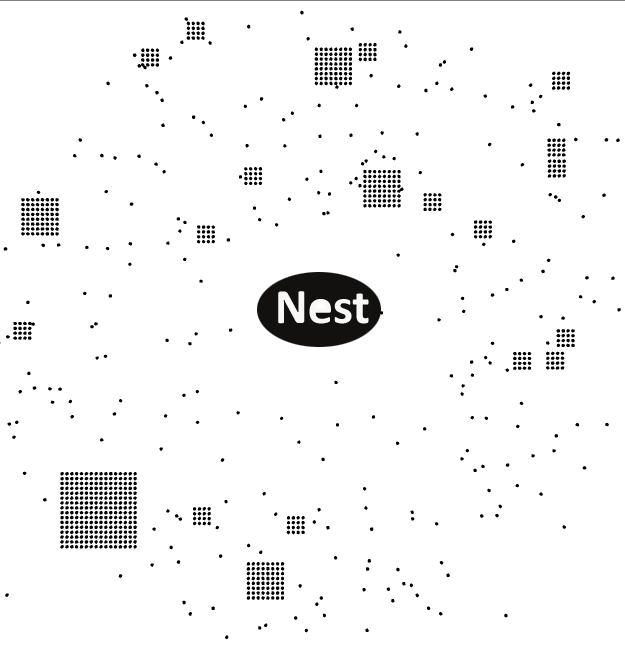
\includegraphics[width=\textwidth]{ArGOS.jpg}}
	\caption{Example setup of a simulation environment for \textit{P. Rugosus} with total 1024 seeds. The setup showing three different types of piles. One large pile of $256$ seeds, Four piles of $64$ seeds and sixteen piles of $16$ seeds. $256$ random seeds are distributed uniformly inside the ring. }
\end{figure}
\section{\label{section:Tuning Parameters using Genetic Algorithm}Tuning Parameters using Genetic Algorithm}
   To analyze the data, we have tuned the parameters of CPFA. As stated above in the background study, enormous amount of parameters for CPFA can be used to evaluate the fitness. But we have used the genetic algorithm to achieve the optimum set of parameters. We have divided the simulations into three categories to tune the GA for three different environments. 
   \begin{enumerate}
   	\item \textbf{Pheromone Only Parameters:}  For this type we have restricted the use of site fidelity. Which means that the probability of using site fidelity is $20$. Rest of the parameters evolved using the GA. 
   	\item \textbf{Site fidelity Only Parameters:} In this types of experiment we restricted the use of pheromone. For this case ants can only use site fidelity and random walk to collect resources
   	\item \textbf{Using Both site fidelity and pheromone:} This environment represents the actual field experiment condition. Here agents use both site fidelity and pheromone along with the random walk.    	
   \end{enumerate}
For each type of environment, we have tuned the parameters to obtain maximum fitness using Genetic Algorithm. Initially, we have created the one hundred set of parameters. And then evaluated their fitness. The best genome is selected for crossover and mutation for next generation. We continued this process until we obtain the best fitness genome or parameter set. The GA is terminated either when the parameters are converged, or it reaches to generation $50$.  
For each parameter set in a population, fitness is tested for four different random seeds. The Random seed is the variable which controls the variables of a simulation. After evaluation of each random seed for one parameter set, we have calculated the average seed collection to define the fitness of that particular set of parameters. These random seeds are basically numbers which are fixed for each generation. For each generation, we have selected four different numbers for the random seeds and then evaluated all the parameters for those values.
For GA we can confine particular parameters to a certain range of values by setting this in evolver.cpp file. For Example, for "Pheromone Only" Environment we restricted the values of site fidelity to $(20,20)$ where each value inside the parenthesis represents upper bound and lower bound.
To calculate the fitness for each parameter set it takes evaluating the fitness function for four times due to four different random seeds, which means for each generation it needs evaluating the objective function for $400$ times. So over $50$ generations, it will need $2000$ evaluations of the objective function. This can take a lot of time if we perform the evaluation sequentially. To remove this bottleneck, we have used multi-threading of genetic algorithm by evaluating multiple objective functions simultaneously. We have used GA Lib Genetic Algorithm Package. The software for this work used the GAlib genetic algorithm package, written by Matthew Wall at the Massachusetts Institute of Technology. The MPI version was written by Andrew Rasmussen \url{https://github.com/andyras/GAlib-mpi/blob/master/LICENSE} who modified the code from \url{https://github.com/B0RJA/GAlib-mpi}.
The evolver.cpp file is used to initialize the GA parameters and pipe the parameters to the GA Lib.
Detail of initial parameter settings of Genetic Algorithm for three different setup is given in the following table.
\begin{table}[h]
	\begin{tabular}{ |p{0.22\textwidth}|p{0.22\textwidth}|p{0.22\textwidth}|p{0.22\textwidth}| } 
		\hline
		\textbf{CPFA Parameters} & \textbf{Pheromone Only} & \textbf{Sitefidelity Only} & \textbf{All Parameters} \\
		\hline 
		Probability of Switching to Searching & U(0,1) & U(0,1) & U(0,1)\\ 
		\hline
		Probability of Returning to Nest & U(0,1) & U(0,1) & U(0,1)\\ 
		\hline
		Uniform Search Variation & (0, 4 PI) & (0, 4 PI) & (0, 4 PI)\\
		\hline
		Rate of Informed Searched Decay & E(20,0) & E(20,0) & E(20,0)\\
		\hline
		Rate of Site Fidelity & E(20,20) & E(20,0) & E(20,0)\\
		\hline
		Rate of Laying Pheromone & E(20,0) & E(20,20) & E(20,0)\\
		\hline
		Rate of Pheromone Decay & E(20,0) & E(20,20) & E(20,0)\\
		\hline
	\end{tabular}
	\caption{Initialization of seven parameters of CPFA for three different environments}
\end{table}
\section{\label{section:Generating Data Set for Analysis}Generating Data Set for Analysis}
 Once the parameters are tuned for three different environments, we have generated the data for our analysis using these parameter sets. For each of the experiment, we have extracted pick up and drop off time for each seed, location of each seed in the arena. Pick up time represents the time when the seed is picked by the ant from the location of the seed and drop time is when it is dropped off at the nest. We have tagged each ant with distinct ID. For each seed, we also have extracted which ant has collected that seed. Also, we have tracked when the pheromone is laid, and followed, and when the site fidelity is followed. We have assigned distinct ID number to each pile so that when a pheromone trail is laid we can track which pile the trail is coming from. For each type of environment, we have simulated $500$ experiments and generated data mentioned above. We varied the value of random seed for each experiment while keeping the CPFA parameters constant for a particular environment. We also varied the position of seeds for each experiment. Each experiment was performed for $90$ minutes. While generating the data for "Pheromone only parameters", We did not extract any site fidelity data, because we tuned all the parameters not to use site fidelity data. Similarly, for "site fidelity only" experiments we did not extract any pheromone data as there was no pheromone. We have collected both site fidelity data and pheromone data when we have used both methods together for collecting resources.
 \section{\label{Analyzing The Foraging Data}Analyzing The Foraging Data}
 After generating all the data from the simulation we have tried to observe how the ants collect seeds from different food distributions. We observed that it takes some time for them to discover the larger piles. But once they discover it, they start to collect seeds from those piles. And they use site fidelity and pheromone for this recruitment. Once they start collecting this seeds we see an increase in their foraging rate. So we tried to detect those changes in their foraging rate by applying the change point detection algorithm. 
 \subsection{\label{Creating Timeline for each type of distribution}Creating Timeline for each type of distribution}
 We have studied each experiment separately to analyze the change in their foraging rate. For each experiment, we studied foraging rate for each type of pile individually. To study foraging rate for each pile we have created a timeline for each type of distribution. 
 \begin{figure}[h]
 	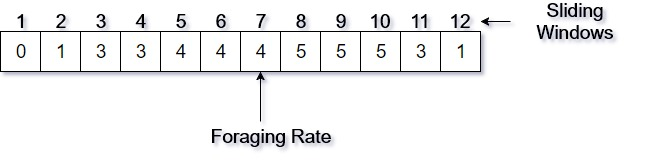
\includegraphics[width=\textwidth]{TimeLine.jpg}
 	\caption{An example of a timeline for a distribution where numbers at the top represent the sliding window number. Values in the boxes are the rate of collection of seeds per window.}
 \end{figure}
 For example, we have divided the whole time of the experiments into sliding windows. Where each sliding window represents the rate of collection of seeds for that time. The length of the sliding window is $60$ seconds for \textit{P. Rugosus}. And then we slided the window by $10$ seconds so that we can get the rate of collecting seeds by that window. So if the experiment is for $90$ minutes ($5400$ seconds), we kept the length of the sliding windows for $60$ seconds and slided it by $10$ seconds, we get total $540$ sets of data where we calculated their foraging rate for a particular pile. Once we have created the timeline for each experiment for a particular distribution of seeds we used Change point detection algorithm to detect the change in the rate of collection of seeds. Another method we have created the timeline is by taking into consideration the change in the rate of foraging. In this method for creating the timeline instead of foraging rate, we take into consideration the change in foraging rate.\\ 
 The length of the window and the sliding amount for the window is different for each species. We have systematically varied this two parameters to fine tune the change point detection algorithms. Values for each of the parameters will be discussed further in the result section. 
 \begin{figure}[h]
 	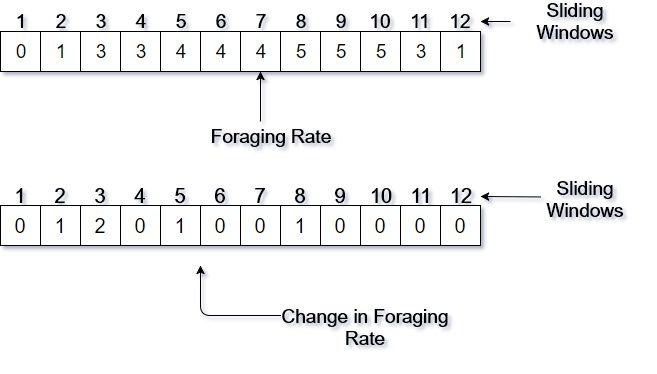
\includegraphics[width=\textwidth]{ChangeInForagingRate.jpg}
 	\caption{An example of timeline and change in foraging rate. The change in foraging rate is calculated by measuring the difference between the timeline windows}
 \end{figure}
\section{\label{section:Change Point Detection Algorithm}Change Point Detection Algorithm}
 The change point detection algorithm is divided into two parts. First part is the adding rate of collecting seeds to calculate the cumulative sum and detrend for smoothing. And the second part is applying the change point detection algorithm. We have used binary segmented cumulative sum method to determine the change points.
 \subsection{\label{Calculating the Cumulative Sum}Calculating the Cumulative Sum}
 The calculation of cumulative sum is basically adding the foraging rate in each window. The following figure and algorithm show how the cumulative sum is calculated.
 \begin{figure}[h]
 	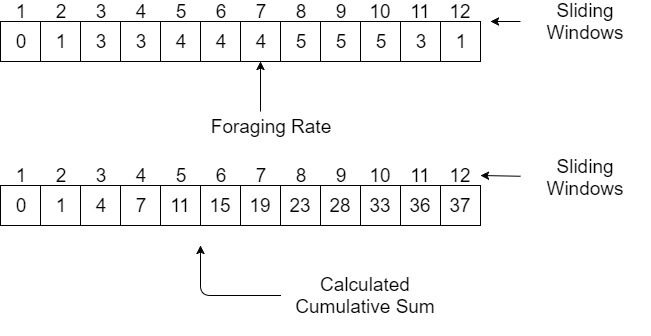
\includegraphics[width=\textwidth]{CumulativeSum.jpg}
 	\caption{This figure demonstrates how the cumulative sum is calculated from the timeline of foraging rate.}
 \end{figure}

 \begin{algorithm}[H]
 	\begin{algorithmic}[1]
 		\State Sum=0
 		\For{i=1:Number of Sliding Window} 
 			\State Sum= Sum + window(i)
 			\State CumulativeSum(i)=Sum
 		\EndFor
 		\caption{Pseudo code for calculating cumulative sum.}
 		\label{Pseudo code for calculating cumulative sum.}
 	\end{algorithmic}
 \end{algorithm}
 
 \subsection{\label{Detrending}Detrending}
 In time series trend means a lazy and gradual change in properties over the whole interval of the event. It is sometimes implicitly defined as a long-term change in the mean. It can also be referred as a change in some statistical properties. Usually, periodic and seasonal components and abrupt fluctuations and other parts were studied separately. Modern analysis techniques frequently treat the series without such routine decomposition, it is still required to consider the trend separately. The removal of a trend in a statistical or mathematical operation of time series is called detrending. It is often applied to remove features which are obsolete or unimportant. In time series analysis, detrending is also used in preprocessing step to prepare data set for further analysis. There are several methods of detrending. Linear trends in mean can be truncated by subtracting a least-square-fit straight line. Different procedures are used for more complicated trend. For example, the cubic smoothing spline is commonly used in dendrochronology to fit and remove ring-width trend that might not be linear, or not even monotonically increasing or decreasing over time. It is important to understand the effect of detrending on spectral properties of time series before trying to remove the trend from the time series. Before applying the change point detection algorithm, we have applied detrending algorithm to remove the trend from the time series. We used linear detrending and constant detrending to observe the effect of detrending in our time series data. Linear detrending removes the linear trend from the data where constant detrending removes the mean from the data. Here is an example, which shows how linear and constant detrending affects the time series.
 \begin{figure}[h]
 	\begin{subfigure}{\textwidth}
 		\centering
 		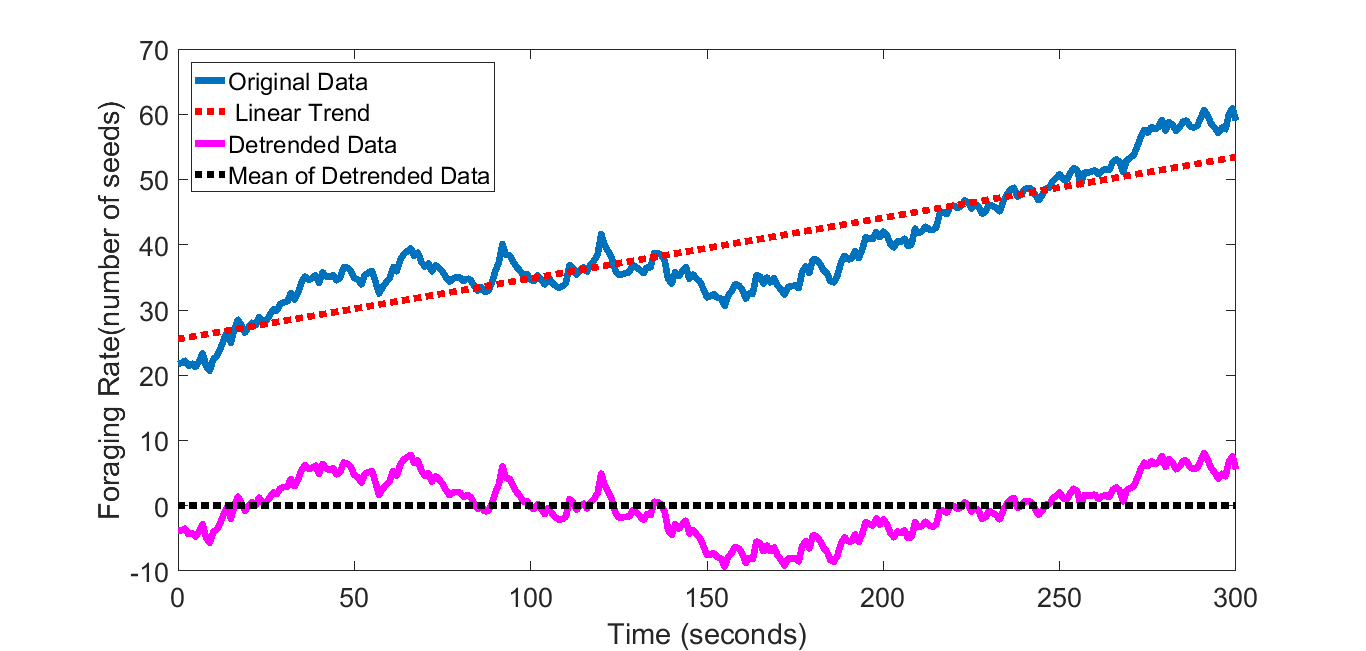
\includegraphics[width=\linewidth]{linearDetrending.jpg}
 		\caption{Linear Detrending}
 		\label{fig:Linear}
 	\end{subfigure}%
 \\
 	\begin{subfigure}{\textwidth}
 		\centering
 		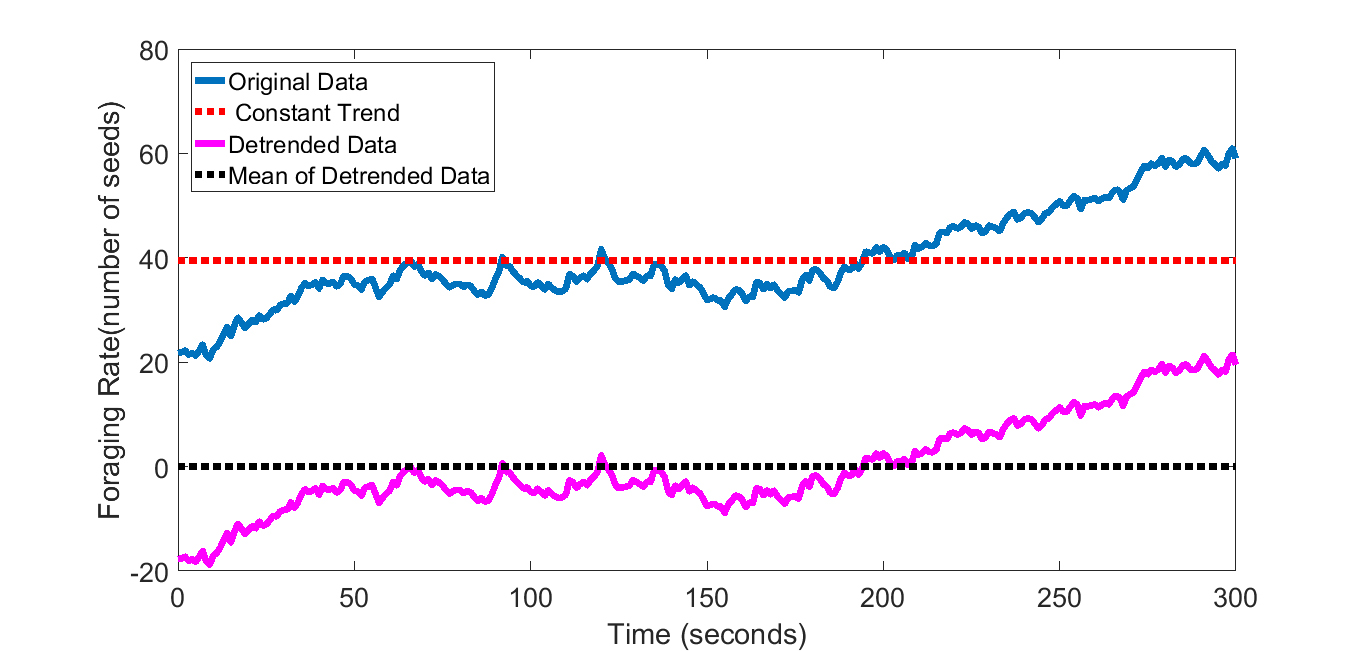
\includegraphics[width=\linewidth]{constantDetrending.jpg}
 		\caption{Constant Detrending}
 		\label{fig:Constant}
 	\end{subfigure}
 	\caption{An example of applying linear and constant detrending on the cumulative sum of a timeline from one simulated CPFA experiment.}
 	\label{fig:fig}
 \end{figure}
\section{\label{section:Binary-Segmented Cumulative Sum}Binary-Segmented Cumulative Sum}
Binary Segmentation is one of the most established search method used for detecting the change point. This method extends any single change point method to multiple change points by iteratively repeating the method on different subsets of the sequence. 
To perform binary segmentation, we first apply the chosen single change point detection method to the entire data set, if no change point is found then we are done. If a change point is detected, call this τ, then the data is split into two segments, timeline$[1:t]$ and timeline$[t+1:n]$. We then apply the single change point method to the two segments and repeat iteratively. We stop when no more change points are detected. 
\\Binary segmentation is a very fast algorithm with complexity $O(n\log n)$ to detect the changes. But the major disadvantage of its computational correctness is that it gives us only an approximation of changes. It is not guaranteed that the binary segmentation method will find us the optimum solution. Also due to iterative nature of this algorithm, it may not detect changes in small changes. Which is why to verify the how well this method is performing, we have verified the results with the simulated data. 
The pseudo code for the binary segmentation algorithm is given in Algorithm $3.2$. 

\begin{algorithm}[!h]
	\begin{algorithmic}[1]
		 \State \algorithmicrequire A set of data of the form ($value_1$,$value_2$,$value_3$...)\\
		\qquad\quad\enspace A test statistic $\tau(.)$\\
		\qquad\quad\enspace An estimator of the changepoint position $\tau(.)$\\
		\qquad\quad\enspace A rejection threshold $\beta$
		\State\textbf{Initialize:} Let $C=\phi$, and $S=[1:n]$
		\While {$S\neq\phi$}
			\State Choose an element of S
			\State Denote this element as $[s,t]$
			\If{$ \tau (ys:t)<\beta $}
				\State remove$[s,t] from S$
			\EndIf
			\If {$\tau(ys:t)\geq\beta$}
				\State remove$[s,t] from S$
				\State calculate $ r=\tau(ys:t)+s-1 $, 
				\State add r to C
				\If {$r\neq s$}
					\State add $[s,r]$ to $S$
				\EndIf
				\If {$r=t-1$}
					\State $[r+1,t]$ to $S$
				\EndIf
			\EndIf
		\EndWhile	
		\caption{Pseudocode for Binary Segmented Mean Cumulative Sum}
		\label{Pseudocode for Binary Segmented Mean Cumulative Sum}
	\end{algorithmic}
\end{algorithm}

\section{\label{section:Verification of Change Points}Verification of Change Points}
As we have simulated data, and we know when the pheromones and site fidelity are used in simulations we can certainly verify how efficient is our change points detection algorithms are. So to check how efficient is our algorithms to detect change points, we divided the detection of change points into 4 categories.
\begin{itemize}
	\item \textbf{Catagory A:} Change point detection within 10 seconds of pheromone laying events, 
	\item \textbf{Catagory B:} Change point detections within 11-300 seconds of pheromone laying events, 
	\item \textbf{Catagory C:} Change point detections after more than 300 seconds of pheromone laying events and 
	\item \textbf{Catagory D:} Change point detected but no pheromone laying events has happened. 
\end{itemize} 
%So we have compared the results of four different methods based on this 4 categories using the data extracted from our simulation.
\section{\label{section:Applying the Best method on Field Data}Applying the Best method on Field Data}
We applied change point detection on 4 different types of the data set. This lead us to evaluate the performance of change point detection algorithm for four different methods.
\begin{figure}[h]
	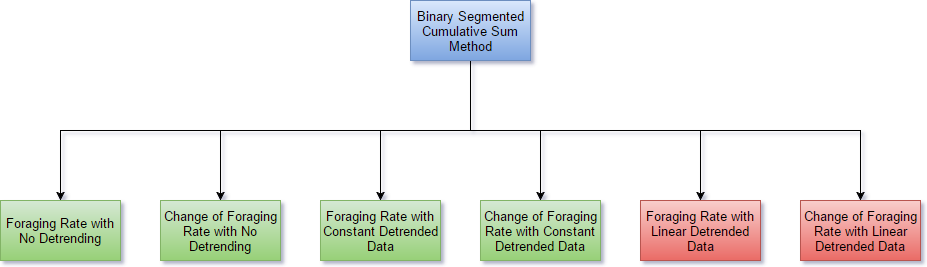
\includegraphics[width=\textwidth]{ChangePoint.png}
	\caption{Four Different Change point Detection Method}
\end{figure}
After validating four different methods that we have applied to simulation data. We select the best method for them based on the performance on four categories stated above. And apply the best method in our field data.   

